\documentclass[12pt,a4paper]{scrartcl}

\usepackage[english]{babel}
\usepackage[T1]{fontenc}
\usepackage{graphicx, subfig}
\usepackage[document]{ragged2e}
\usepackage{lmodern}
\usepackage{color}
\usepackage{amsmath}
\usepackage{graphicx}
\usepackage{amsmath}
\usepackage{amsfonts}
\usepackage{amssymb}

% Für Verwendugn von Utnerstrichen ohne Escaping
\usepackage{underscore}

% Für Referenzen mit eigenem Text
\usepackage{hyperref}

% Für Codeblöcke
\usepackage{listings}

% Für Verwendung von Farben
\usepackage[usenames,dvipsnames,svgnames,table]{xcolor}

% Für Verktor-Pfeile
\usepackage{esvect}

% Für Größe der Seitenränder
\usepackage[margin=1in,footskip=0.5in]{geometry}

% Für Tabellen über Seiten hinweg
\usepackage{longtable}

% Für Header and Footer
\usepackage[automark]{scrpage2}

% Für Bildunterschriften
\usepackage[aboveskip=2pt]{caption}

% Formatierung für Hyperref-Referenzen
\hypersetup{
	colorlinks,
	linkcolor={blue!50!black},
	citecolor={blue!50!black},
	urlcolor={blue!80!black}
}

% Generelle Formatierung für Code-Blöcke
\lstset{ %
	columns=fullflexible,
	keepspaces=true,
	frame=single,
	breaklines=true,
	breakautoindent=true,
	gobble=0,
	tabsize=2,
	belowskip=0pt
}

% Formatierung für Pseudo-Code
\lstdefinelanguage{PSEUDO} 
{ 
	xleftmargin=0pt, 
	xrightmargin=0pt,
	basicstyle=\small\ttfamily\color{Black},
	morekeywords={for, each, if, else},	
	keywordstyle = {\color{Orange}},
	sensitive=false,
	morecomment=[l]{//},
	morecomment=[s]{/*}{*/},
	morestring=[b]"
}

\newcommand{\mybox}{%
    \collectbox{%
        \setlength{\fboxsep}{1pt}%
        \fbox{\BOXCONTENT}%
    }%
}
\makeatother
\title{Water simulation in OpenGL}
\author{Fabian Niehaus, Tuyet Nguyen}
\date{Juni 22, 2018}

\makeatletter

%% Generelle Kopf- und Fußzeilendefinition
\pagestyle{scrheadings}
%\automark[section]{subsection} 
\clearscrheadfoot
\ihead[]{\@title}
%\ohead[]{\rightmark}
\ifoot[]{\@author}

\begin{document}

\begin{titlepage}
	\centering
	\ \\[2cm]
	{\huge\textbf{\@title}} 
	\\[3cm]
	\large
	\textbf{Field of study:} Media informatics \\
	\textbf{Semester:} 4
	\\[2cm]
	\textbf{Date}: \@date
	\\[2cm]
	\textbf {Authors:}
	\\Fabian Niehaus
	\\Tuyet Nguyen
\end{titlepage}

\newpage
%% Seitezahl auf 0 setzen
\setcounter{page}{0}
\tableofcontents
\newpage
\listoffigures

\newpage
%% Seitennummern einblenden
\ofoot[]{\pagemark}
\normalsize

\section{Abstract}
In this project we will build a C++ application to simulate circular waves on a 3D mesh surface. We will also simulate reflection using the Image Source Method. We will use QT Creator for programming, QT for window management and OpenGL for 3D rendering.

\section{Wave theory}
An obvious way to represent waves is through sine or cosine functions. If one chooses the parameters wavelength, amplitude and wave direction with a certain variance around specified basic values and superimposes a number of these waves, this results in at least one water-like wave train. The following formula results for a sum of sine waves, which are visualized by the Heigth Field H. The water is at rest in the x / z plane of a coordinate system.\\

This results in an altitude value in the height field for each position (x, z), with the amplitude a, the direction vector D and a phase shift φ. D stands parallel to the stationary water surface and perpendicular to the associated wave train and the phase velocity c, the frequency f and the so-called wave number k are defined by \\

c =g·l 2π \\
f = c/l\\
k = 2π /l\\

with the wavelength l and the gravitational acceleration g = 9,81m / s2. \\

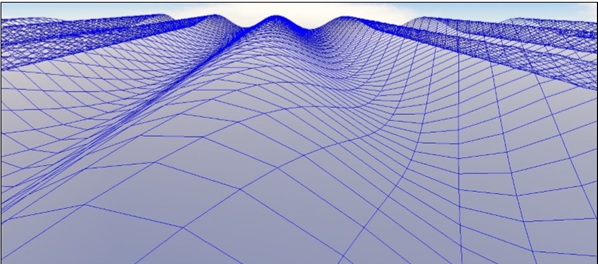
\includegraphics[width=0.7\textwidth]{Images/SinWaves.jpg}

\section{Realisation}

\subsection{Creating a basic interface with QT}
First off, we create a new QT widget application. This allows us to use QT Creators design feature to set up our application's interface. A new QOpenGLWidget is placed and will be used as a placeholder for a new custom class inheriting QOpenGLWidgets functionality. This class, called OGLWidget, needs to implement the following methods: initializeGL (for setting up OpenGL), paintGL (for doing the actual rendering), resizeGL (for handling resizes of the display window). Additionally, the functions stepAnimation SetMaterialColor and InitLightingAndProjection\footnote{Taken from Prof. Dr. Martin Hering-Bertrams OpenGL_Example} are used.

\subsection{Creating the data structure}
The data structure is separated in different classes. \\
The basic class "Waves" contains the contains the information of the waves like sine waves, Height-Field, coordinate, direction vector, phase velocity, the frequency and the wave number.  \\ 
The class "Wavesurface" contains the wavesfunction . 
Logic and data regarding the computation of quad meshes is stored in a seperate class, as are Bezier surfaces and rotational sweep surfaces. \\
In order to allow for easier use of a two dimensional matrix of vertices, a wrapper class containing a two dimensional vector of vertices is introduces. \\


\subsection{Creating the surface mesh}
After creating the required data structure, a method to make a mesh for the waves.\\
Custom data structure\\
2-dimensional vector of QVector3D\\
Dimensions: 50 x 50 -> Best result\\

\subsection{Calculating the wave height}
\begin{lstlisting}[language=PSEUDO]
double distanceToOrigin = QVector2D(x,z).distanceToPoint(wave.O);

double phi = -2 * wave.pi * wave.f * (time + wave.timeOffset);

y += wave.a * cos(wave.k * distanceToOrigin + phi) / (distanceToOrigin + 1);

\end{lstlisting}

\captionof{figure}{Determining adjacent quads (pseudo code)} 

\begin{lstlisting}[language=PSEUDO]
F = exp( i*abs(X*2*pi/8.5))
freq = 10;

for t=0:.001:1
phi = -2*pi*freq*t
F1 = exp( i* phi) * F;
plot( X, real(F1));
axis([-50 50 -5 5]);
drawnow
end


\end{lstlisting}

\captionof{figure}{Determining adjacent quads (pseudo code)} 

\subsection{Rendering as a wireframe}
Depending on the desired way of rendering the object, different draw methods are implemented. These methods are then being called from the paintGL() function.

\subsection{Rendering as an opaque surface}
After drawing the object as a wireframe we want to draw it as a solid cube with lighting. This is being achieved in the method drawQuads() which once again iterates over the list of quads. This time using GL_Quads, the four vertices of a quad are connected and the area inbetween is filled. The normal vector for this is calculated using the cross product of the two diagonals vectors.

\subsection{Reflection}
\begin{lstlisting}[language=PSEUDO]
// Benachbarte Ursprungspunkte berechnen
        QVector2D n1 = QVector2D(-1 * meshDim_X - sourceX, meshDim_Z - sourceZ); // links oben
        QVector2D n2 = QVector2D(sourceX, meshDim_Z - sourceZ); // oben
        QVector2D n3 = QVector2D(meshDim_X - sourceX, meshDim_Z - sourceZ); // rechts oben
        QVector2D n4 = QVector2D(-1 * meshDim_X - sourceX, sourceZ); // links
        QVector2D n5 = QVector2D(meshDim_X - sourceX, sourceZ); // rechts
        QVector2D n6 = QVector2D(-1 * meshDim_X - sourceX, -1 * meshDim_Z - sourceZ); // links unten
        QVector2D n7 = QVector2D(sourceX, -1 * meshDim_Z - sourceZ); // unten
        QVector2D n8 = QVector2D(meshDim_X - sourceX, -1 * meshDim_Z - sourceZ); // rechts unten

        // Urpsungspunkt ausgeben für Debugging
        cout << "N1: " << n1.x() << " | " << n1.y() << endl;
        cout << "N2: " << n2.x() << " | " << n2.y() << endl;
        cout << "N3: " << n3.x() << " | " << n3.y() << endl;
        cout << "N4: " << n4.x() << " | " << n4.y() << endl;
        cout << "N5: " << n5.x() << " | " << n5.y() << endl;
        cout << "N6: " << n6.x() << " | " << n6.y() << endl;
        cout << "N7: " << n7.x() << " | " << n7.y() << endl;
        cout << "N8: " << n8.x() << " | " << n8.y() << endl;

        // Wellen mit entsprechenden Ursprungspunkten einfügen
        waveSurface->addWave(Wave (amplitude, wavelength, 0.0, n1));
        waveSurface->addWave(Wave (amplitude, wavelength, 0.0, n2));
        waveSurface->addWave(Wave (amplitude, wavelength, 0.0, n3));
        waveSurface->addWave(Wave (amplitude, wavelength, 0.0, n4));
        waveSurface->addWave(Wave (amplitude, wavelength, 0.0, n5));
        waveSurface->addWave(Wave (amplitude, wavelength, 0.0, n6));
        waveSurface->addWave(Wave (amplitude, wavelength, 0.0, n7));
        waveSurface->addWave(Wave (amplitude, wavelength, 0.0, n8));



\end{lstlisting}

\captionof{figure}{Determining adjacent quads (pseudo code)} 
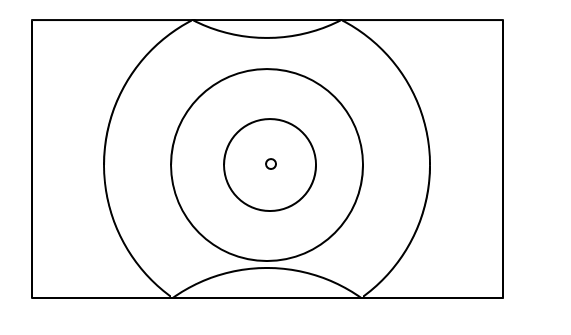
\includegraphics[width=0.7\textwidth]{Images/Reflextion.png}


\subsection{Fazit}
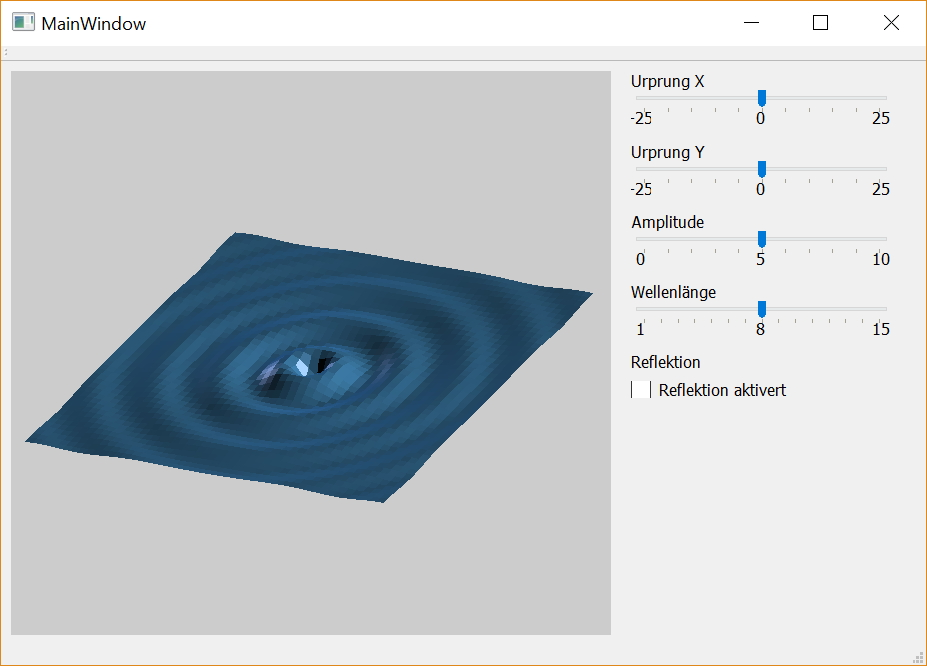
\includegraphics[width=0.7\textwidth]{Images/Wave1.jpg}
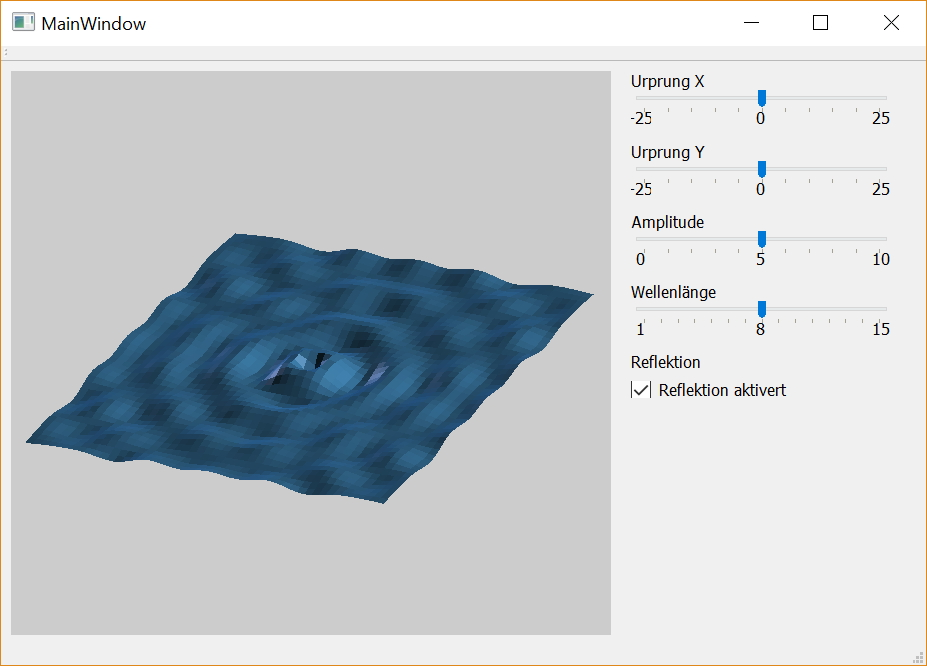
\includegraphics[width=0.7\textwidth]{Images/WavewithReflextion.jpg}
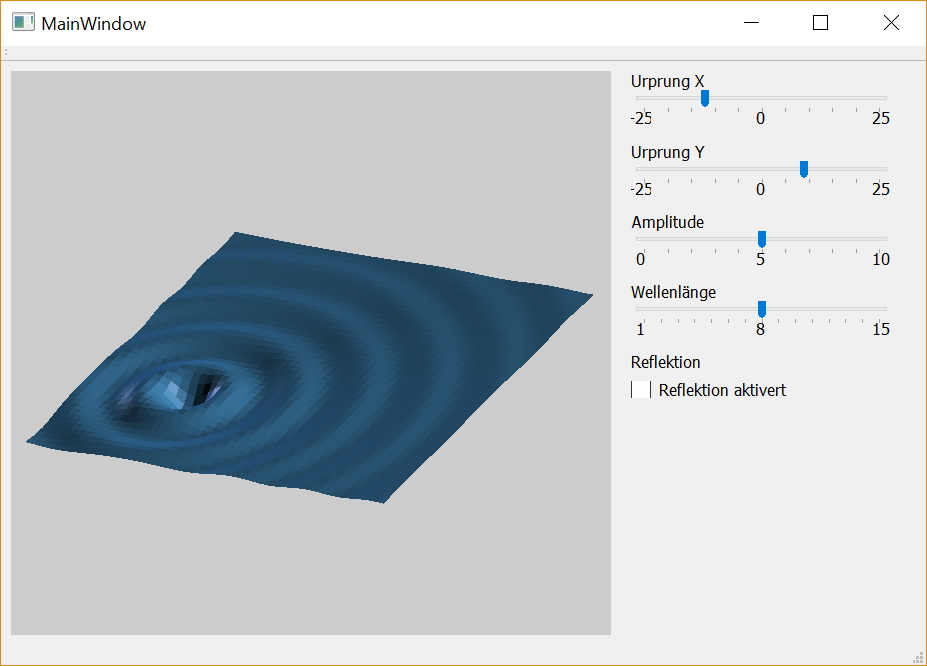
\includegraphics[width=0.7\textwidth]{Images/xAndy.jpg}
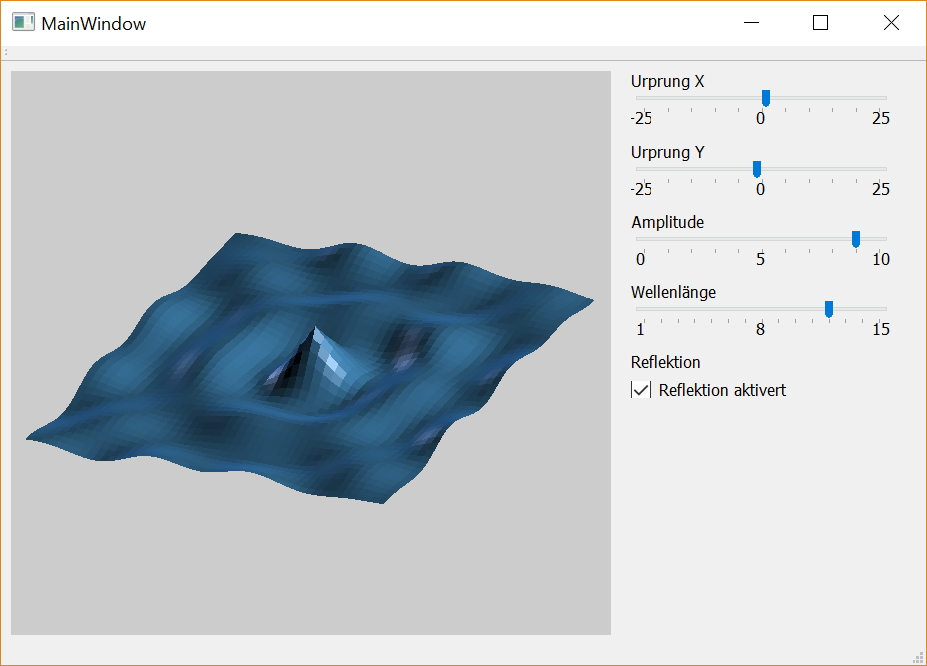
\includegraphics[width=0.7\textwidth]{Images/HighaAndl.jpg}

\end{document}